\documentclass[a4paper,12pt]{article}
%%%%%%%%%%%%%%%%%%%%%%%%%%%%%%%%%%%%%%%%%%%%%%%%%%%%%%%%%%%%%%%%%%%%%%%%%%%%%%%%%%%%%%%%%%%%%%%%%%%%%%%%%%%%%%%%%%%%%%%%%%%%%%%%%%%%%%%%%%%%%%%%%%%%%%%%%%%%%%%%%%%%%%%%%%%%%%%%%%%%%%%%%%%%%%%%%%%%%%%%%%%%%%%%%%%%%%%%%%%%%%%%%%%%%%%%%%%%%%%%%%%%%%%%%%%%
\usepackage{eurosym}
\usepackage{vmargin}
\usepackage{amsmath}
\usepackage{graphics}
\usepackage{epsfig}
\usepackage{subfigure}
\usepackage{fancyhdr}
\usepackage{listings}
\usepackage{framed}
\usepackage{graphicx}
\usepackage{amsmath}
\usepackage{chngpage}
%\usepackage{bigints}


\setcounter{MaxMatrixCols}{10}

\begin{document}
\begin{center}
       
\includegraphics[scale=0.55]{shieldtransparent2}
\end{center}

\begin{center}
\vspace{1cm}
\large \bf {FACULTY OF SCIENCE AND ENGINEERING} \\[0.5cm]
\normalsize DEPARTMENT OF MATHEMATICS AND STATISTICS \\[1.25cm]
\large \bf {END OF SEMESTER EXAMINATION PAPER 2015} \\[1.5cm]
\end{center}

\begin{tabular}{ll}
MODULE CODE: MA4505 & SEMESTER: Autumn 2015 \\[1cm]
MODULE TITLE: Applied Statistics for Administation & DURATION OF EXAM: 2.5 hours \\[1cm]
LECTURER: Mr. Kevin O'Brien & GRADING SCHEME: 100 marks \\[1cm]
ASSESSORS: Dr. M.F. Brezzo & C.F. Ryback \\[1cm]
& \phantom{GRADING SCHEME:} \footnotesize {70\% of module grade} \\[0.8cm]
\\[1cm]
\end{tabular}
\begin{center}
{\bf INSTRUCTIONS TO CANDIDATES}
\end{center}

{\noindent \\ Scientific calculators approved by the University of Limerick can be used. \\
Formula sheet and statistical tables provided at the end of the exam paper.\\
There are 5 questions in this exam. Students must attempt any 4 questions.}
\newpage



% - Section 1 Inference Procedures
        % a. Parametric
        % b. Non Parametric
% - Section 2 Linear Models
        % a. SLR
        % b. MLR
% - Section 3 Linear Models
        % a. Robust Regression
        % b. AIC
% - Section 4 Statistical Process control
        % a. Control Limits
        % b. Theory Questions
        % c. Interpreting Charts
        % d. CUSUM and ARL
% - Section 5 Experimental Design 1
        % a. Definitions for ED
        % b. One Way ANOVA
% - Section 6 Experimental Design 2
        % a.
        % b.
\subsection*{Question 1. Inference Procedures - (Variant A) }
\subsubsection*{Part A : Inference Procedures}

The reproducibility of a method for the determination of a pollutant in water was investigated by
taking twelve samples from a single batch of water and determining the concentration of pollutant
in each. The following results were obtained:\[ 5.98, 8.80, 6.89, 8.49, 8.48, 7.47, 7.97, 6.94, 7.32, 6.64,
6.98, 7.94. \]
It is expected that from this sample a 95\% confidence interval for the concentration of
pollutant will be obtained.
\begin{itemize}
\item[(i)] There is a concern that the data may contain an outlier. Thus the following procedure has been
performed on the data (which is simply referred to a X in the code output):
\begin{framed}
\begin{verbatim}
Dixon test for outliers
data: X
Q = 0.3625, p-value = 0.6326
alternative hypothesis: lowest value 5.98 is an outlier
\end{verbatim}
\end{framed}
\begin{itemize}
\item[$\bullet$] (2 Marks) Describe what is the purpose of this procedure.
\item[$\bullet$] (1 Mark) Write the conclusion that follows from it.
\end{itemize}

\item[(ii)] After the test for an outlier, another preliminary procedure has been performed on the data
\begin{framed}
	\begin{verbatim}
Anderson-Darling normality test

data:  X
A = 0.24067, p-value = 0.7132
\end{verbatim}
\end{framed}
\begin{itemize}
	\item[$\bullet$] (2pts) Explain what is the name and purpose of this procedure. State the null and alternative hypothesis used for this procedure.
\item[$\bullet$] (1pts) What is the conclusion and why?
\end{itemize}
\newpage
\item[(iii)] After these initial verifications, the confidence interval can be obtained from the following computations
Based on the obtained values write down the confidence interval for the pollutant. 
\begin{framed}
\begin{verbatim}
t = 1.9868, df = 11, p-value = 0.07242
alternative hypothesis: true mean is not equal to 7
95 percent confidence interval:
6.946999 8.036334
sample estimates:
mean of x 
7.491667 
\end{verbatim}
\end{framed}
\end{itemize}
\newpage
\subsection*{Question 1. Inference Procedures - (Variant B) }
\subsubsection*{Part A : Inference Procedures}
\begin{itemize}
\item The nicotine content in blood can be determined by gas chromatography down to concentrations of 1 ng/ml. The concentration of nicotine was determined in each of two samples of known concentrations 10 ng/ml and 50 ng/ml.
\begin{framed}
\begin{verbatim}
Data: Sample (Lo): m = 10 ng/ml, n=14.

 8.40, 9.59, 9.38, 9.10, 10.78, 11.41, 9.94, 
10.08, 12.11, 9.10, 9.59, 10.36, 10.41, 10.52.

Data: Sample (Hi): m = 50 ng/ml, n=10.

47.5, 48.4, 48.8, 48.4, 46.8, 
46.2, 48.6, 50.6, 45.5, 46.1.
\end{verbatim}
\end{framed}
A research team evaluated both samples to determine whether or not the samples were similar in terms of measures of centrality and dispersion, before the trial commenced.  \\  \\ The following blocks of \texttt{R} code (i.e blocks 1 to 6) are based on the data for this assessment. \\ 
\begin{itemize}
\item[(a)] (3 Marks) Each of the six blocks of code describes a statistical inference procedure. Provide a brief description for each procedure.
\item[(b)] (4 Marks) Write a short report on your conclusion for this assessment, clearly indicating which blocks of \texttt{R} code you felt were most relevant, and explain why. 
\end{itemize}

\begin{itemize}
\item[\textbf{Block 1}]
\begin{framed}
\begin{verbatim}

        F test to compare two variances

data:  Lo and Hi
F = 0.3945, num df = 13, denom df = 9, p-value = 0.1246
alternative hypothesis: 
 true ratio of variances is not equal to 1
95 percent confidence interval:
 0.1029905 1.3066461
sample estimates:
ratio of variances 
         0.3945149
\end{verbatim}
\end{framed}

\item[\textbf{Block 2}]
\begin{framed}
\begin{verbatim}
> shapiro.test(Lo)

        Shapiro-Wilk normality test

data:  Lo
W = 0.9779, p-value = 0.9609
> shapiro.test(Hi)

        Shapiro-Wilk normality test

data:  Hi
W = 0.9496, p-value = 0.6634
\end{verbatim}
\end{framed}
\bigskip
\item[\textbf{Block 3}]
\begin{framed}
\begin{verbatim}
> t.test(Lo,Hi)

        Welch Two Sample t-test

data:  Lo and Hi
t = -67.374, df = 14.016, p-value < 2.2e-16
alternative hypothesis: 
   true difference in means is not equal to 0
95 percent confidence interval:
 -38.83294 -36.43706
sample estimates:
mean of x mean of y 
   10.055    47.690 
\end{verbatim}
\end{framed}
\newpage
\item[\textbf{Block 4}]
\begin{framed}
\begin{verbatim}
> t.test(Lo,Hi,var.equal=TRUE)

        Two Sample t-test

data:  Lo and Hi
t = -72.6977, df = 22, p-value < 2.2e-16
alternative hypothesis: 
   true difference in means is not equal to 0
95 percent confidence interval:
 -38.70863 -36.56137
sample estimates:
mean of x mean of y 
   10.055    47.690 

\end{verbatim}
\end{framed}



\item[\textbf{Block 5}]
\begin{framed}
\begin{verbatim}
> ks.test(Lo,Hi)

        Two-sample Kolmogorov-Smirnov test

data:  Lo and Hi
D = 1, p-value = 1.02e-06
alternative hypothesis: two-sided

\end{verbatim}
\end{framed}
%------------------------------------------------------------------%
\item[\textbf{Block 6}]
\begin{framed}
\begin{verbatim}
 wilcox.test(Lo,Hi)

        Wilcoxon rank sum test


data:  Lo and Hi
W = 0, p-value = 1.02e-06
alternative hypothesis: 
	true location shift is not equal to 0

\end{verbatim}
\end{framed}
\end{itemize}

\end{itemize} % End of Question Block
%--------------------------------------------------------------------------------------------------------%
%--------------------------------------------------------------------------------------------------------%

\newpage
\newpage
%Q2A Simple Linear Linear Regression
%Q2B Method Comparison Studies
\subsection*{Question 1. Inference Procedures - (Variant C) }
\subsubsection*{Part A : Outliers}
\begin{itemize}
\item (3 Marks) Provide a brief description for three tests from the family of Grubb's  Outliers Tests. Include in your description a statement of the null and alternative hypothesis for each test, any required assumptions and the limitations of these tests.
\item (3 Marks) Showing your working, use the Dixon Q Test to test the hypothesis that the maximum value of the following data set is an outlier.
\[ 19,22,23,24,25,26,29,38\]
\end{itemize}	

\newpage
\subsection*{Question 2. Linear Models - (Variant A) }
%--------------------------------------------------------------------------------------------------------%
%\begin{itemize} %Start of Question
	
	
	%-------------------------------Start of Question 2A%
	
%	\item[(a)]
	The fluorescence of each of a series of acidic solutions of quinine with concentrations 0,10,20,30,40,50
	was determined five times. The mean values and standard deviations of these determinations have
	been obtained as follows:
	\begin{center}
		\begin{tabular}{|c|cccccc|}
			\hline
			% after \\: \hline or \cline{col1-col2} \cline{col3-col4} ...
			Means: & 4.0 & 21.2& 44.6& 61.8& 78.0 &105.2\\
			Std Deviations: &0.71& 0.84 &0.89 &1.64 &2.24 &3.03\\
			\hline
		\end{tabular}
	\end{center}
	Two models have been fitted to the data. These models are described by the following \texttt{R} code output.
	
	
	\subsubsection*{Model 1}
		\begin{framed}
			
			
			
			\begin{verbatim}
			lm(formula = Means ~ Conc)
			
			Coefficients:
			Estimate Std. Error t value Pr(>|t|)
			(Intercept) 2.9238 2.1648 1.351 0.248
			Conc 1.9817 0.0715 27.715 1.01e-05 ***
			---
			Residual standard error: 2.991 on 4 degrees of freedom
			Multiple R-squared: 0.9948,Adjusted R-squared: 0.9935
			F-statistic: 768.1 on 1 and 4 DF, p-value: 1.008e-05
			\end{verbatim}
		\end{framed}
		\subsubsection*{Model 2}
		\begin{framed}
		
			\begin{verbatim}
			weights=SdInt^(-2)/mean(SdInt^(-2))
			
			lm(formula = Means ~ Conc, weights = weights)
			Coefficients:
			Estimate Std. Error t value Pr(>|t|)
			(Intercept) 3.48066 1.15736 3.007 0.0397 *
			Conc 1.96315 0.06765 29.018 8.4e-06 ***
			---
			Residual standard error: 2.034 on 4 degrees of freedom
			Multiple R-squared: 0.9953,Adjusted R-squared: 0.9941
			F-statistic: 842 on 1 and 4 DF, p-value: 8.396e-06
			\end{verbatim}
		\end{framed}
	\begin{itemize}
		%\item[i.] (2 marks) What is the regression equation for this fitted model?
		%\item[ii.] (4 marks) Comment on the significance of the regression estimates.
		\item[i.] (4 Marks) What kind of analyses have been performed in each of model 1 and model 2? Write down the linear model regression equation fitted by each of the two analyses.
		
		\item[ii.] (3 Marks) Describe differences between the two models, making reference to the scatter-plot of the data on the next page. (Also present on the scatter-plot is a regression line fitted using the first analysis).
		\item[iii.] (2 Marks) Based on the \texttt{R} code output, which model is the better fit?
		%\item[iv.] (2 Marks) What is the Akaike information criterion? Descibe how it could be used in this context.
	\end{itemize}
	\newpage
	\begin{center}
		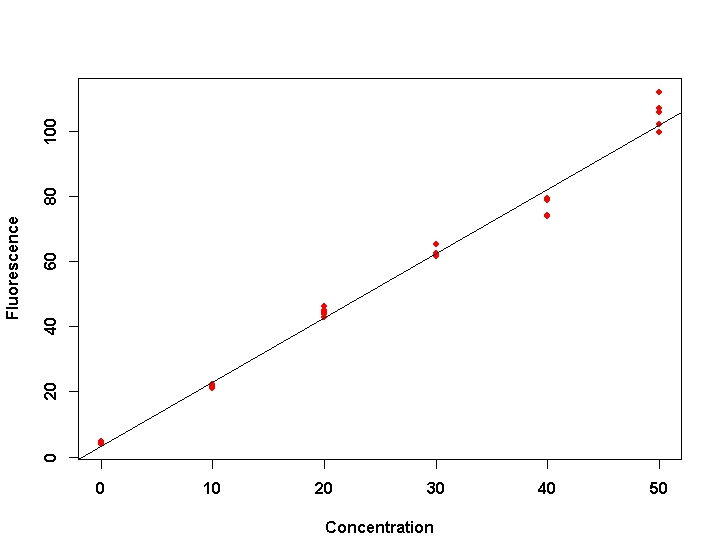
\includegraphics[scale=0.45]{ExamQ2plot2}
	\end{center}.
	%\begin{center}
	%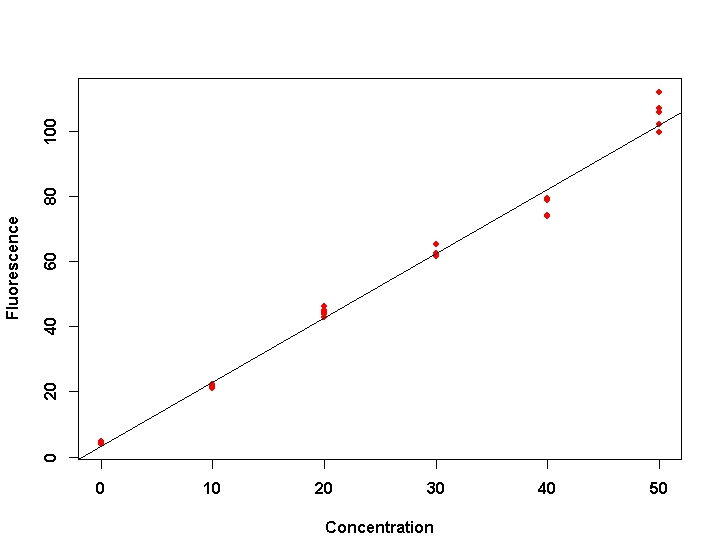
\includegraphics[scale=0.60]{ExamQ2plot2}
	%\end{center}
\newpage
\subsection*{Question 2. Linear Models - (Variant B) }
	%-------------------------------End  of Question 2A%
(4 Marks) Complete the following \textit{Analysis of Variance} Table for a simple linear regression model based on the data provided. The required values are indicated by question marks.
\begin{center}
\begin{tabular}{|c|c|c|c|c|c|} \hline
           & Df & 	Sum Sq &	Mean Sq &	F value &   	Pr($>$F)    \\ \hline
Regression &  ? &	9160239 &	? &	 ? &	$< 2.2e^{-16}$ \\ \hline
    Error  & 50 &	2134710 &  	?   &            &       \\ \hline
    Total  & ?  &	? &  	42694   &            &       \\ \hline
\end{tabular} 
\end{center}

Once you have completed this table, compute the following
\begin{itemize}
	\item (1 Mark)  The Pearson correlation coefficient for the response variable Y and the predictor variable X.
	\item (1 Mark) Tthe sample standard deviation of the response variable Y.
\end{itemize}

\newpage

\subsection{Question 2. Linear Models (Variant C)}
Problem 1 (20pts)
The following results were obtained when each of a series of standard silver solutions was analysed by
ame atomic-absorption spectrometry. The analysis of these by means of R is also presented below.
\begin{figure}[h!]
\centering
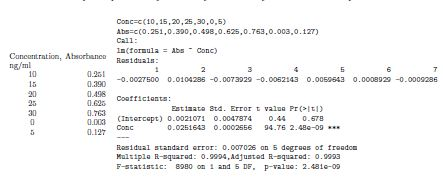
\includegraphics[width=1.1\linewidth]{Sample1}
\caption{}
\label{fig:Sample1}
\end{figure}

Based on this information do the following
(3pts) Determine the slope and intercept of the calibration plot and make a sketch of the linear fit to
the date. Include data points on the graph as well.
(2pts) Determine the 95\% confidence limits for the slope and intercept. (The corresponding quantiles
of Student t-distribution are given by qt(0:025; 5) = 􀀀2:57 and qt(0:975; 5) = 2:57.)
(4pts) Based on the above calibration fit find the silver concentration for a sample giving an absorbance
of 0.42 in a single determination. Estimate the 95\% confidence limits for the silver concentration.
The following formula for the standard deviation of the concentration determination should be
used for the purpose
\begin{figure}[h!]
\centering
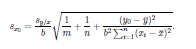
\includegraphics[width=0.5\linewidth]{Sample2}
\end{figure}

The following computations in R allows for effective computation of the above standard deviation

\begin{framed}
\begin{verbatim}
> mean(Abs)
[1] 0.3795714
> mean(Conc)
[1] 15
> sum((Conc-mean(Conc))^2)
[1] 700
\end{verbatim}
\end{framed}
\begin{itemize}
\item (6pts) Find the silver concentration for a sample giving absorbance values of 0.30, 0.31, 0.29 in three
separate analyses of the same sample. Estimate the confidence limits for the concentration in
this case. How the accuracy improved comparing to the one in the previous question? (In your
computations you should use the information from the previous question.)
\item (5pts) Estimate the limit of detection of the silver analysis.
\end{itemize}
\newpage
\subsection*{Question 3. ANOVA and Experimental Design (Variant A)}

% Definitions
% One Way ANOVA
% Checking Assumptions

\begin{itemize}
	\item[(a)] Explain the following terms in the context of experimental design
	\begin{itemize}
		\item[i.] (1 Mark) levels of a factor.
		\item[ii.] (1 Mark) randomized block design.
	\end{itemize}

\item[(b)] Six analysts each made seven determinations of the paracetamol content of the same batch of tablets.
The results are shown in the table below. In the last two columns are the sample means and standard deviations for each sample.\\
\bigskip

\begin{tabular}{|c|ccccccc|c|c|}
\hline
Group &  & &  &  &  &  &  & $\bar{X}$& $S_{X}$ \\ \hline
A & 84.32 & 84.51 & 84.63 & 84.61 & 84.64 & 84.51 & 84.62 & 84.5486 & \\ \hline
B & 84.24 & 84.25 & 84.41 & 84.13 & 84.00 & 84.30 & 84.02 & 84.1928 & \\ \hline
C & 84.29 & 84.40 & 84.68 & 84.28 & 84.40 & 84.36 & 84.63 & 84.4342 & \\ \hline
D & 84.14 & 84.22 & 84.02 & 84.48 & 84.27 & 84.33 & 84.22 & 84.2400 & \\ \hline
E & 84.50 & 83.88 & 84.49 & 83.91 & 84.11 & 84.06 & 83.99 & 84.1343 & \\ \hline
F & 84.70 & 84.17 & 84.11 & 84.36 & 84.61 & 83.81 & 84.15 & 84.2729 & \\ \hline
\end{tabular} 


\bigskip

For the aggregrate sample (all 42 observations) the standard deviation is $0.2381$.

\begin{itemize}
\item[(i)] (5 Marks) Complete the following One Way Analysis of Variance Table.
\item[(ii)] (1 Marks) Describe what is the purpose of this procedure. include a statement of the null and alternative hypothesis in your answer.
\item[(iii)] (2 Marks) (5 Marks)
\end{itemize}
\begin{tabular}{|r|c|c|c|c|c|}
	\hline Source  &\phantom{sp} DF \phantom{sp} & Sum Squares & Mean Square  & \phantom{sp} F \phantom{sp} & p-value  \\ 
	\hline Between-Groups &  &  &  &  & 0.003941 \\ 
	\hline Within-Groups &  &  &  &  &  \\ \hline
	\hline Total &  &  &  &  &  \\ 
	\hline 
\end{tabular} 



\end{itemize}

\newpage	
\subsection*{Question 3. ANOVA and Experimental Design (Variant B) }
\begin{itemize} % Start of Question 5
	\item[(a)] % Part A
	
	In an investigation into the extraction of nitrate-nitrogen from air dried soil, three quantitative variables were investigated at two levels. These were the amount of oxidised activated charcoal (A) added to the extracting solution to remove organic interferences, the strength of CaSO4 extracting solution (C), and the time the soil was shaken with the solution (T). The aim of the investigation was to optimise the extraction procedure. The levels of the variables are given here:
	\begin{center}
		{
			\large
			\begin{tabular}{|cc|c|c|}
				\hline	&		&\phantom{sp}	{\LARGE -}\phantom{sp}	&	\phantom{sp} {\LARGE +} \phantom{sp}	\\ \hline
				Activated charcoal (g) 	&	A 	&	0.5	&	1	\\ \hline
				CaSO{4} (\%) 	&	C 	&	0.1	&	0.2	\\ \hline
				Time (minutes) 	&	T 	&	30	&	60	\\ \hline
			\end{tabular} 
		}
	\end{center}
	
	The concentrations of nitrate-nitrogen were determined by ultra-violet spectrophotometry and compared with concentrations determined by a standard technique. The results are given below and are the amounts recovered (expressed as the percentage of known nitrate concentration).
	{
		\large
		\begin{center}
			\begin{tabular}{|c|c|c|cc|}
				\hline
				\phantom{sp}A\phantom{sp}	&	\phantom{sp}C\phantom{sp}	&\phantom{sp}	T\phantom{sp}	&	Amounts&	(2 Replicates)	\\
				\hline
				-1	&	-1	&	-1	&	45.1	&	44.6	\\ \hline
				
				1	&	-1	&	-1	&	44.9	&	45.3	\\ \hline
				
				-1	&	1	&	-1	&	44.8	&	46.7	\\ \hline
				
				1	&	1	&	-1	&	44.7	&	44.8	\\ \hline
				
				-1	&	-1	&	1	&	33	&	35	\\ \hline
				
				1	&	-1	&	1	&	53.8	&	51.7	\\ \hline
				
				-1	&	1	&	1	&	32.6	&	33.7	\\ \hline							
				1	&	1	&	1	&	54.2	&	53.2	\\ \hline
			\end{tabular}
		\end{center}
	}
\end{itemize}


\newpage


\begin{itemize}
	\item[i.] (6 Marks) Calculate the contrasts, the effects and the sum of squares for the effects.
	\item[ii.] (4 Marks) Using the computed sums of squares values, complete the ANOVA table (see the \texttt{R} code below).
	\item[iii.] (2 Marks) Comment on the tests for significant for the main effects and interactions. State clearly your conclusions.
	\item[iv.] (3 Marks) Write down a  regression equation that can be used predicting amounts based on the results of this experiment.
\end{itemize}

{
\large
\begin{framed}
	\begin{verbatim}
	            Df Sum Sq Mean Sq F value     Pr(>F)    
	A            1    ...     ...     ...   0.000979 ***
	C            1    ...     ...     ...   0.934131    
	T            1    ...     ...     ...   0.395554 
	A:C          1    ...     ...     ...   0.944243    
	A:T          1    ...     ...     ...   0.017582 *
	C:T          1    ...     ...     ...   0.072101
	A:C:T        1    ...     ...     ...   0.028522 *    
	Residuals    8  116.2    14.5                      
	\end{verbatim}
\end{framed}
}

\newpage
(Find the NEW plots)
\begin{center}
	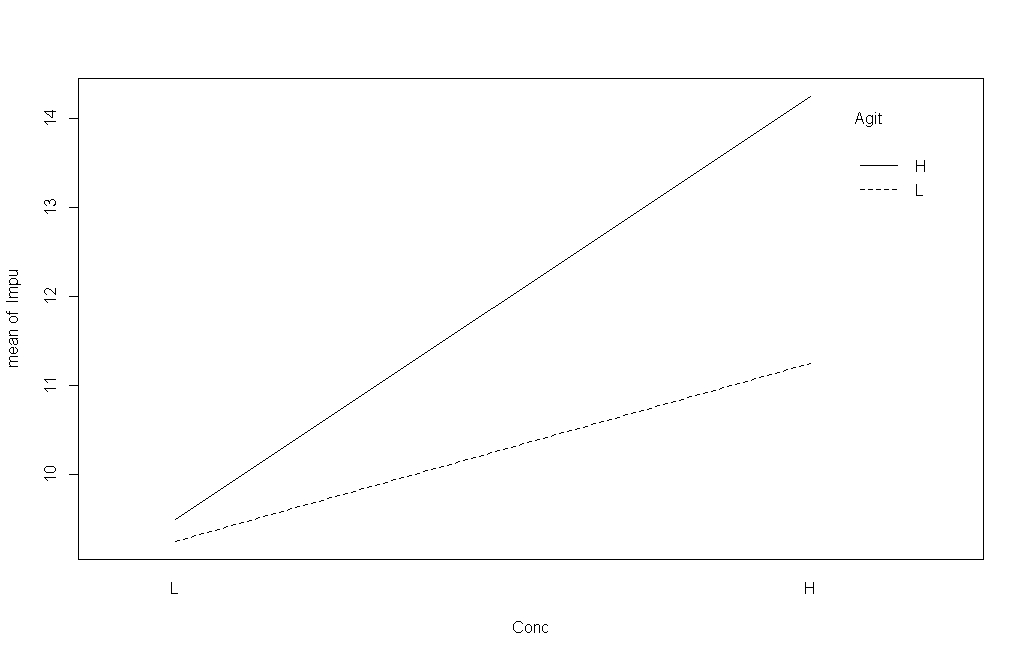
\includegraphics[scale=0.24]{image/ExamQ6interactiona}
\end{center}
\begin{center}
	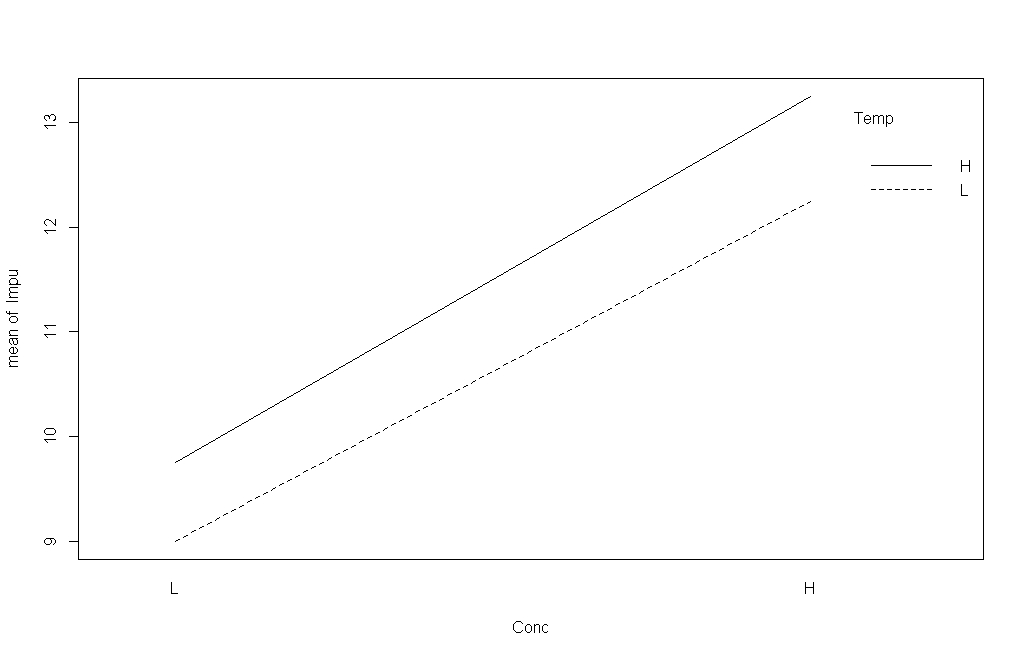
\includegraphics[scale=0.24]{image/ExamQ6interactionb}
\end{center}
\begin{center}
	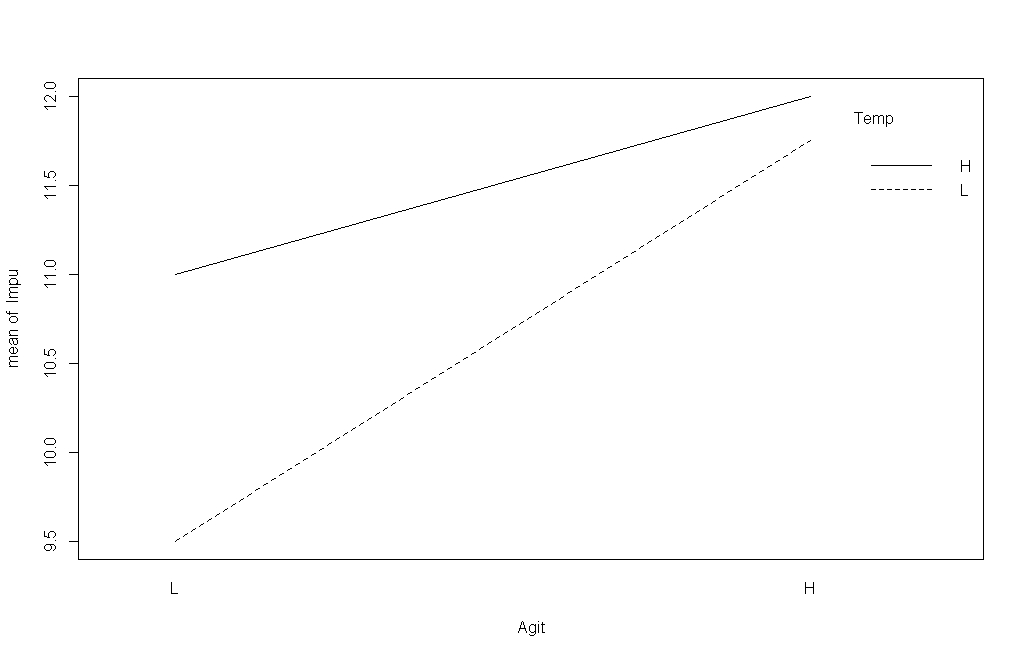
\includegraphics[scale=0.24]{image/ExamQ6interactionc}
\end{center}
\newpage
\subsection*{Question 5. Statistical Process Control (Variant A) }




\begin{itemize}
	\item[(a)] Answer the following questions.
	
	\begin{itemize}
		\item[i] (1 marks) Differentiate common causes of variation in the quality of process output from assignable causes.
		\item[ii.] (1 marks) What is tampering in the context of statistical process control?
		\item[iii] (2 marks) Other than applying the \emph{Three Sigma} rule for detecting the presence of an assignable cause, what else do we look for when studying a control chart? Support your answer with sketches.
	\end{itemize}
	
	\item[(b)] A normally distributed quality characteristic is monitored through the use of control charts. These charts have the following parameters. All charts are in control.
	\begin{center}
		\begin{tabular}{|c|c|c|c|}
			\hline  & LCL & Centre Line & UCL \\
			\hline $\bar{X}$-Chart & 542 & 550 & 558 \\
			\hline $R$-Chart & 0 & 8.236 & 16.504 \\ \hline
		\end{tabular}
	\end{center}
	
	\begin{itemize}
		\item[i] (2 marks) What sample size is being used for this analysis?
		\item[ii.] (2 marks) Estimate the standard deviation of this process.
		\item[iii.] (2 marks) Compute the control limits for the process standard deviation chart (i.e. the s-chart).
	\end{itemize}
	
	\item[(c)] An automobile assembly plant concerned about quality improvement measured sets of five camshafts on twenty occasions throughout the day. The specifications for the process state that the design specification limits at 600$\pm$3mm.
	
	
	\begin{itemize}
		\item[i.] (3 marks) Determine the \emph{Process Capability Indices} $C_p$ and $C_{pk}$, commenting on the respective values. You may use the \texttt{R} code output on the following page.
		\item[ii.] (1 marks)  The value of $C_{pm}$ is $1.353$. Explain why there would be a discrepancy between $C_p$ and $C_{pm}$.
		\item[iii.] (1 marks) Comment on the graphical output of the \emph{Process Capability Analysis}, also presented on the next page.
	\end{itemize}
	
	
	\newpage
	\begin{framed}
		\begin{verbatim}
		Process Capability Analysis
		
		Call:
		process.capability(object = obj, spec.limits = c(597, 603))
		Number of obs = 100          Target = 600
		Center = 599.548         LSL = 597
		StdDev = 0.5846948       USL = 603
		
		Capability indices:
		Value   2.5%  97.5%
		Cp    ...
		Cp_l  ...
		Cp_u  ...
		Cp_k  ...
		Cpm   1.353  1.134  1.572
		Exp<LSL 0%   Obs<LSL 0%
		\end{verbatim}
	\end{framed}
	
	
	
	\begin{center}
		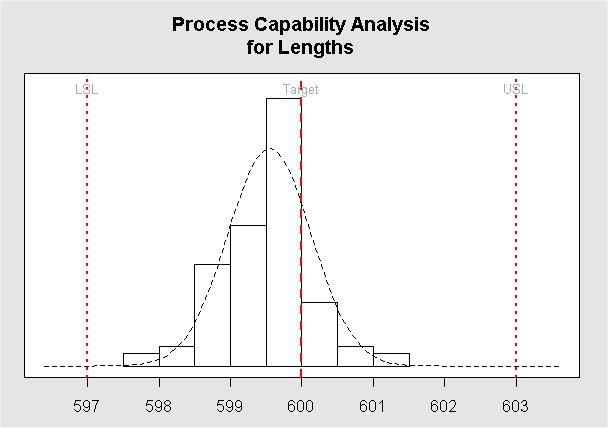
\includegraphics[scale=0.55]{image/ExamQ4hist}
	\end{center}
	\newpage
	%
	%Lengths = Values
	%
	%obj <- qcc(Lengths, type="xbar")
	%
	%process.capability(obj, spec.limits=c(597,603))
\end{itemize}

\newpage
\subsection*{Critical Values for Dixon Q Test}
\begin{center}
	\begin{tabular}{|c|c|c|c|}
		\hline  N  & $\alpha=0.10$  & $\alpha=0.05$  & $\alpha=0.01$  \\ \hline
		3  & 0.941 & 0.97  & 0.994 \\ \hline
		4  & 0.765 & 0.829 & 0.926 \\ \hline
		5  & 0.642 & 0.71  & 0.821 \\ \hline
		6  & 0.56  & 0.625 & 0.74  \\ \hline
		7  & 0.507 & 0.568 & 0.68  \\ \hline
		8  & 0.468 & 0.526 & 0.634 \\ \hline
		9  & 0.437 & 0.493 & 0.598 \\ \hline
		10 & 0.412 & 0.466 & 0.568 \\ \hline
		11 & 0.392 & 0.444 & 0.542 \\ \hline
		12 & 0.376 & 0.426 & 0.522 \\ \hline
		13 & 0.361 & 0.41  & 0.503 \\ \hline
		14 & 0.349 & 0.396 & 0.488 \\ \hline
		15 & 0.338 & 0.384 & 0.475 \\ \hline
		16 & 0.329 & 0.374 & 0.463 \\ \hline
	\end{tabular} 
\end{center}

\subsection*{Process Capability Indices}
\[ \hat{C}_p = \frac{\mbox{USL} - \mbox{LSL}}{6s}\]

\[ \hat{C}_{pk} = \mbox{min} \left[\frac{\mbox{USL} - \bar{x}}{3s},\frac{\bar{x} - \mbox{LSL}}{3s} \right] \]

\[ \hat{C}_{pm} = \frac{\mbox{USL} - \mbox{LSL}}{6\sqrt{s^2+(\bar{x}-T)^2}}\]
\bigskip
%\subsection*{2^3 Design: Main Effect}
%
%\[X= \frac{1}{4n} \left[ x + xy + xz + xyz - (1) - y - z - yz \right]\]
%\bigskip
\subsection*{$2^3$ Design: Interaction Effects}

\[ AB = \frac{1}{4n} \left[ abc - bc + ab - b - ac + c - a + (1) \right] \]

\[ AC = \frac{1}{4n} \left[ (1) - a + b - ab -c + ac - bc + abc \right] \]

\[ BC = \frac{1}{4n} \left[ (1) + a - b - ab - c - ac + bc + abc \right] \]

\[ABC = \frac{1}{4n} \left[ abc - bc - ac + c - ab + b +  a - (1) \right] \]

\bigskip

\subsection*{Factorial Design: Sums of Squares}

\[\mbox{Effect} =  \frac{\mbox{(Contrast)}}{n2^{k-1}}\]

\[\mbox{Sums of Squares} =  \frac{\mbox{(Contrast)}^2}{n2^k}\]

%------------------------------------------------------------------------ %
\Large{
	\subsection*{Factors for Control Charts}
	\begin{tabular}{|c|c|c|c|c|c|c|}
		\hline
		Sample Size (n) 	&	c4 	&	c5 	&	d2 	&	d3 	&	D3 	&	D4	\\	\hline
		2	&	0.7979	&	0.6028	&	1.128	&	0.853	&	0	&	3.267	\\	
		3	&	0.8862	&	0.4633	&	1.693	&	0.888	&	0	&	2.574	\\	
		4	&	0.9213	&	0.3889	&	2.059	&	0.88	&	0	&	2.282	\\	
		5	&	0.9400	&	0.3412	&	2.326	&	0.864	&	0	&	2.114	\\	
		6	&	0.9515	&	0.3076	&	2.534	&	0.848	&	0	&	2.004	\\	
		7	&	0.9594	&	0.282	&	2.704	&	0.833	&	0.076	&	1.924	\\	
		8	&	0.9650	&	0.2622	&	2.847	&	0.82	&	0.136	&	1.864	\\	
		9	&	0.9693	&	0.2459	&	2.970	&	0.808	&	0.184	&	1.816	\\	
		10	&	0.9727	&	0.2321	&	3.078	&	0.797	&	0.223	&	1.777	\\	
		11	&	0.9754	&	0.2204	&	3.173	&	0.787	&	0.256	&	1.744	\\	
		12	&	0.9776	&	0.2105	&	3.258	&	0.778	&	0.283	&	1.717	\\	
		13	&	0.9794	&	0.2019	&	3.336	&	0.770	&	0.307	&	1.693	\\	
		14	&	0.9810	&	0.1940	&	3.407	&	0.763	&	0.328	&	1.672	\\	
		15	&	0.9823	&	0.1873	&	3.472	&	0.756	&	0.347	&	1.653	\\	
		16	&	0.9835	&	0.1809	&	3.532	&	0.750	&	0.363	&	1.637	\\
		17	&	0.9845	&	0.1754	&	3.588	&	0.744	&	0.378	&	1.622	\\
		18	&	0.9854	&	0.1703	&	3.64	&	0.739	&	0.391	&	1.608	\\
		19	&	0.9862	&	0.1656	&	3.689	&	0.734	&	0.403	&	1.597	\\
		20	&	0.9869	&	0.1613	&	3.735	&	0.729	&	0.415	&	1.585	\\
		21	&	0.9876	&	0.1570	&	3.778	&	0.724	&	0.425	&	1.575	\\
		22	&	0.9882	&	0.1532	&	3.819	&	0.720	&	0.434	&	1.566	\\
		23	&	0.9887	&	0.1499	&	3.858	&	0.716	&	0.443	&	1.557	\\
		24	&	0.9892	&	0.1466	&	3.895	&	0.712	&	0.451	&	1.548	\\
		25	&	0.9896	&	0.1438	&	3.931	&	0.708	&	0.459	&	1.541	\\
		\hline
	\end{tabular}
} % End Large Font

\end{document}


%======================================================================= %
\section{R Code for Part 3}
\begin{verbatim}
ALL <- c(84.32, 84.51, 84.63, 84.61, 84.64, 84.51, 84.62, 84.24, 84.25, 
84.41, 84.13, 84, 84.3, 84.02, 84.29, 84.4, 84.68, 84.28, 84.4, 
84.36, 84.63, 84.14, 84.22, 84.02, 84.48, 84.27, 84.33, 84.22, 
84.5, 83.88, 84.49, 83.91, 84.11, 84.06, 83.99, 84.7, 84.17, 
84.11, 84.36, 84.61, 83.81, 84.15)

\end{verbatim}